\documentclass[a4paper,10pt]{article}
\usepackage[utf8x]{inputenc}
\usepackage{verbatim}
\usepackage{graphicx}
\usepackage{enumerate}

%opening
\title{Lab 3}
\author{William Richard}

\begin{document}

\maketitle

\section{p139 E5.2}
\begin{enumerate}[(a)]
  \item The output of top or ps, sorted by cpu usage or memory usage, quickly and easily reveal processes that are hogging resources.
  \item 
\begin{verbatim}
kill -s STOP -p <pid>
\end{verbatim}
  \item 
\begin{verbatim}
kill -s CONT -p <pid>
\end{verbatim}
  \item I would send the TERM signal - this allows the process to die gracefully.
\begin{verbatim}
kill -s TERM -p <pid>
\end{verbatim}
If I needed to guaranee that the process died, I would send the KILL signal, or signal 9, which forces tho process to die, and does not allow it to try to exit gracefully.
\begin{verbatim}
kill -s KILL -p <pid>
\end{verbatim}
\end{enumerate}

\section{Hands On Lab}
\subsection{ps -ef $|$ grep bash $|$ grep -v grep}
\begin{center}
 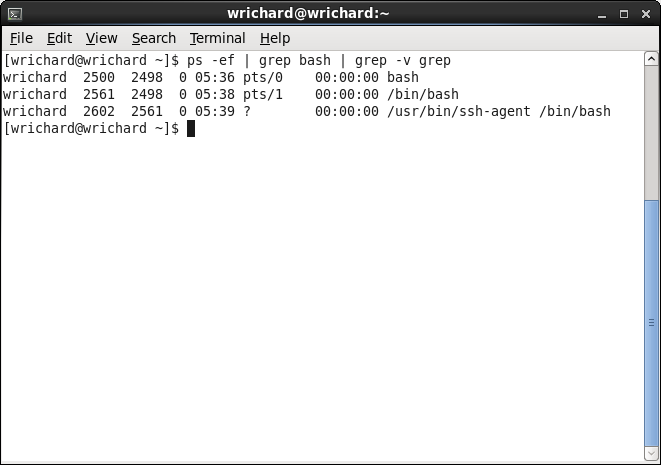
\includegraphics[width=\linewidth]{./grepbash.png}
\end{center}
\subsection{find\_proc.sh}
\subsubsection{Code}
\verbatiminput{find_proc.sh}

\end{document}
